\chapter{Formal rules for three-part counterpoint}\label{chapter:species}
The purpose of this section is to extract all the rules that Fux mentions in his work and to make sure that they are unambiguous.

It consists of seven sections: first, a section for the implicit rules (the rules that Fux doesn't mention, but are present in all his examples), then a section for each species, and finally a short section that considers the interaction between different species. There is no section on rules for all species, yet there \textit{are} rules that apply to all species. In fact, all the rules mentioned in the first species section also apply to the other species. Although Fux doesn't explicitly mention this point, it becomes clear when you look at how he teaches and applies these rules in composition.Therefore, the rules for all species are in the first species section. The reason these rules are in the first type section is because Fux himself mentions these rules in his chapter on first type counterpoint.

Each species section is divided into two subsections: the first subsection is about setting up Fux's rules and discussing them. The second subsection is about translating the rules into formal logic.

\paragraph*{Some important notes}
\begin{itemize}
    \item \textbf{Concerning the green dot} ---
    Please note that all the rules from T. Wafflard's thesis still apply to three-part compositions. The numbering of the rules in this work is the same as in T. Wafflard's work. If a rule is defined with the same number as an existing rule for two-part compositions, this means that the corresponding rule from T. Wafflard's work does not apply to three-part compositions, and that the new rule should be used instead. To make this clearer, there is a green dot (\greendot) next to the rules from T. Wafflard's thesis that got redefined when used in a three-voice composition.
    \item \textbf{Concerning the \texttt{[PREF]} marker} ---
    As discussed earlier (see Section~\ref{subsection:preferences-vs-hard-rules}), some rules are mandatory and must be followed to find a valid solution, and other rules are just preferences that can be followed to find a \textit{better} solution. The preferences have been marked '\texttt{[PREF]}' throughout the chapter clearly mark which rule is mandatory and which is a preference.

    \item \textbf{Concerning the default costs} --- Each time a cost is mentioned in the formalisation rules, the value corresponding to it is its default value, as defined in Appendix~\ref{chapter:user-guide}. Note, however, that in practice the value for each cost can be changed by the user to suit their needs.
    \item \textbf{Concerning the purpose of all the rules} --- 
    It may be interesting to remember the purpose of these rules. Some rules are concerned with musicality: composing counterpoint that sounds nice; for example, the rule that forbids dissonance. Some rules are concerned with singability: composing counterpoint that is not too difficult for the human voice to sing; for example, the rule forbidding a melodic leap greater than a sixth.

\end{itemize}

\section{Implicit rules}
These implicit rules apply to all types of counterpoint. They are never explicitly defined by Fux, but are derived from his many examples. These implicit rules are therefore actually used by Fux, even though he doesn't talk about them.

\subsection{Formalisation in English} \label{sec:generalenglish}
\begin{enumerate}[wide, label=\bfseries 1.H2 and 1.H\arabic*]
    \setcounter{enumi}{2} % Start from 8
    \item \greendots \textit{First and last notes have not to be perfect consonances anymore.} \label{rule:last-chord-not-perfect-anymore}    

    Fux doesn't state this in his text, but in many of his examples, we see that when he composes with three voices (and more), the first and last harmonic intervals between the parts and the lowest stratum are not necessary a perfect consonance anymore.
\end{enumerate}

\begin{enumerate}[wide, label=\bfseries 1.H7 and 1.H\arabic*]
    \setcounter{enumi}{7} % Start from 8
    \item \greendots \textit{The harmonic interval of the penultimate measure must be either a minor
    third, a perfect fifth, a major sixth, or an octave.} \label{rule:penult-interval-3-voices}
    
    In two-part composition rules, Fux said that the last harmonic interval had to be either a minor or a majord third (see rule~\ref{rule:penult-interval-2v} for two voices). This is something he doesn't respect at all in three-part composition, but we can see that he still tries to use minor third and major sixths when possible, in the penultimate measure. The rule from two-part species was thus rewritten in order to be appropriate: either use a perfect consonance, a minor third, or a major sixth.
\end{enumerate}

\begin{enumerate}[wide, label=\bfseries G\arabic*]
    \setcounter{enumi}{7} % Start from 8

    \item\label{rule:last-chord-h-triad} \textit{The last chord must be composed only of the notes of the harmonic triad.} 

    Again, this isn't stated explicitly, but we see that all of his examples end with a chord containing exclusively the notes of the harmonic triad.
    
    \item \textit{The last chord must have the same fundamental as the one of the scale used throughout the composition.}\label{rule:same-fundamental}

    This rule emanates from an observation of Fux's examples throughout the chapter. The last chord of all his compositions always have the same fundamental as the fundamental of the scale used throughout the composition.
    When the \textit{cantus firmus} is the lowest stratum, this is not a problem, as the \textit{cantus firmi} always end with the fundamental note of the scale. But when not, it has to be imposed by a constraint, or we may end up with surprising results.
\end{enumerate}

\subsection{Formalisation into constraints} \label{sec:generalconstraints}
    \paragraph{\hspace{0.6cm}\ref{rule:last-chord-not-perfect-anymore}} \greendots \textit{First and last notes have not to be perfect consonances anymore.}

    There is no constraint associated with this rule, as it is a relaxation of a rule from the two-part composition rule set.

    \paragraph{\hspace{0.6cm}\ref{rule:penult-interval-3-voices}} \greendots \textit{The harmonic interval of the penultimate measure must be either a minor third, a perfect fifth, a major sixth, or an octave.}
    \begin{equation}
        \begin{aligned}
            H[0, m-2] \in \{0, 3, 7, 9\}
        \end{aligned}
    \end{equation}

    \paragraph{\hspace{0.6cm}\ref{rule:last-chord-h-triad}} \textit{The last chord must be composed only of the notes of the harmonic triad.} 
    
    \begin{equation} \begin{aligned}
    \forall s \in \{b, c\} \colon H(s)[0, m-1] \in Cons_{h\_triad}
    \end{aligned} \end{equation}

    \paragraph{\hspace{0.6cm}\ref{rule:same-fundamental}} \textit{The last chord must have the same fundamental as the one of the scale used throughout the composition.}\label{constraint:same-fundamental}

    Since the fundamental of the scale is defined by being the first note of the \textit{cantus firmus}, we impose that the last note of the lowest stratum must be equal to the first one of the \textit{cantus firmus} (taking the modulos into account).
    
    
    \begin{equation} \begin{aligned}
    N(a)[0, m-1] \mod 12 = N(\mathit{cf})[0, 0] \mod 12
    \end{aligned} \end{equation}

\section{First species}
This section deals with the rules that apply to the first species of counterpoint. As mentioned earlier, these rules apply to \textit{all} species in the context of a three-part composition. In other words, these rules apply whenever $species(p) \in \{0, 1, 2, 3, 4, 5\}$. More specifically, the rules in this section apply to the first beat of each species, except for the fourth species, where they apply to the third beat (see the note on the fourth species~\ref{nota-bene-4th-species}).

\paragraph{}
The first species consists of whole notes only. It is the basis of counterpoint and its simplest case. 

\begin{figure}[h]
    \centering
    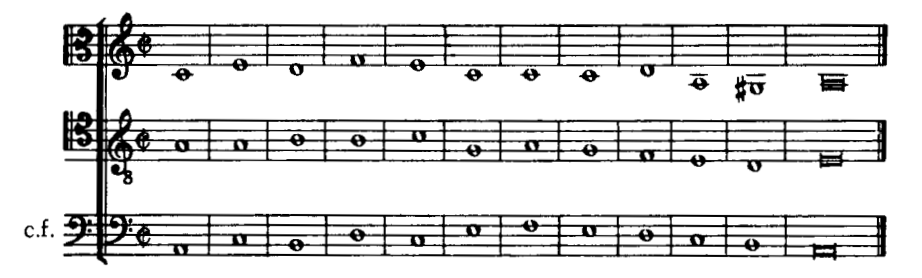
\includegraphics[width=1\textwidth]{Images/Species_examples/1sp-example.png}
    \caption{Example of a first species counterpoint in three-part composition}
    \label{fig:example-1sp}
\end{figure}

\subsection{Formalisation into English}
\subsubsection{Structural constraints}
\begin{enumerate}[wide, label=\bfseries 1.S\arabic*]
    \item\label{rule:allwhole} \textit{All notes are whole notes.}
     
    \begin{quotation}
       "This species consists of three whole notes in each instance."
       \textcite[p.71]{GaPEng}
   \end{quotation}

   This pretty straightforward rule is the very definition of the first species. It adds nothing in comparison with the rules for the two part comparison. It is hence already implemented by the first species for two voices and does not need any consideration. 
\end{enumerate}
\subsubsection{Harmonic rules}
\begin{enumerate}[wide, label=\bfseries 1.H\arabic*]
    \item\label{rule:consonant} \greendots \textit{All notes on the downbeat are consonant with the notes of the lowest stratum.}
     
    \begin{quotation}
       "This species consists of three notes, the upper two being consonant with the lowest."
       \textcite[p.71]{GaPEng}
   \end{quotation}

   This rule is an update of previous \textbf{1.H1} (that previously was saying that \textit{all} intervals must be consonants). Fux states that the upper voices and the lowest one are consonant, and not all voices together. 
    
    \setcounter{enumi}{7} % Start from 8

    \item\label{rule:harmonic-triad} \texttt{[PREF]}  \textit{The harmonic triad should be used as much as possible.} 

    \begin{quotation}
    "The harmonic triad should be employed in every measure if there is no special reason against it."
    \textcite[p.71]{GaPEng}
    \end{quotation}

    As a footnote states it \cite[footnote, p.71]{GaPEng}, Fux refers to the "harmonic triad" as being a chord in this position: 1-3-5 (contrary to what is today understood as a harmonic triad).
    The rule says it is not obligated, but it is preferred, to use the 1-3-5 chord, considering that 1 is the lowest voice.
    

    \item\label{rule:sixth-or-octaves}  \textit{One might use sixths or octaves.}

    \begin{quotation}
    "Occasionally, one uses a consonance not properly belonging to the triad, namely, a sixth or an octave."
    \textcite[p.72]{GaPEng}
    \end{quotation}

    Here, Fux explains that when it is not possible to have a harmonic triad, you can use sixths or octaves instead. Remember that the sixths or the octaves are calculated from the lowest stratum. Since the rule~\ref{rule:consonant} obligates the use of a perfect consonance (i.e. a third, a fifth, a sixth or an octave), when the harmonic triad cannot be used, it is already naturally replaced by a third or a sixth, because no other intervals are allowed. It is thus not a new rule but a restatement of rule~\ref{rule:consonant}.    

    \item\label{rule:tenth-is-last-chord}  \textit{Tenths are prohibited in the last chord.}

    \begin{quotation}
    "One feels that the degree of perfection and repose which is required of the final chord does not become sufficiently positive with this imperfect consonance [(speaking about a tenth)]."
    \textcite[p.77]{GaPEng}
    \end{quotation}

    When Fux says this, he takes a tenth as an example, but it here understood that the final chord cannot include a tenth (third + octave), nor an eight-teenth (third + two octaves), etc. Nevertheless, "simple" third are considered completely valid.

    \item\label{rule:unison-vs-octave} \texttt{[PREF]} \textit{Octaves should be preferred over unisons.}

    \begin{quotation}
    "Unison is less harmonious than the octave."
    \textcite[p.79]{GaPEng}
    \end{quotation}

    This rule does not bring anything new, as there is already a rule stating that two parts cannot blend in unison (\ref{rule:no-unison-appendix}). If no unison is possible, then the octaves will always be preferred over the unison (since the latter is not possible).

    \item\label{rule:minor-third}  \textit{Last chord cannot include a minor third.}

    \begin{quotation}
    "The minor third is not capable of giving a sense of conclusion."
    \textcite[p.80]{GaPEng}
    \end{quotation}

    Fux later states that minor modes should not include a third altogether, but that sometimes it is impossible to do without it, so the major third \textit{is} allowed in minor modes.

\end{enumerate}

\subsubsection{Melodic rules}
The following rules obviously don't apply to the \cf, since its melody is already fixed.
\begin{enumerate}[wide, label=\bfseries 1.M\arabic*]
\setcounter{enumi}{2} % Start from 3
    \item\label{rule:steps-prefered} \texttt{[PREF]} \textit{Steps are preferred to skips.}

    \begin{quotation}
    "[Each part] follows the natural order closely."
    \textcite[p.73]{GaPEng}
    \end{quotation}

    After having said this, Fux complements his explication by saying the counterpoints should be "moving gracefully, stepwise without any skip". This is clearly a preference, and has already been covered when implementing the first species for two voices (see~\ref{rule:smallmelody}). It can thus be ignored in the scope of this thesis.

    \item\label{rule:variety} \texttt{[PREF]}  \textit{The notes of each part should be as diverse as possible.}

    \begin{quotation}
    "[Each part] follows the principle of variety."
    \textcite[p.73]{GaPEng}
    \end{quotation}

    Fux never clearly defines what he means by the "principle of variety". So we try to define it according to what we can read in his work. The examples he gives are a great help. He first writes an incorrect example and then corrects it, saying that the corrected example is better because it follows the principle of variety more closely. The difference between the two examples is that the number of different pitches has been increased. So we can define the principle of variety as: use as many different notes as possible in a single voice. 

    The principle of variety is therefore clearly a preference.

    This principle is very interesting because it introduces the only rule \textit{across all} rules that has a scope greater than two measures. While without this rule the solver uses constraints that apply only to one measure (think of harmonic constraints) or sometimes to two measures (think of melodic constraints), this constraint is the first to give the solver some "memory" about the composition. And although seven measures may seem like a small range, it means that the constraint covers a large part of the composition (when dealing with compositions of 10 to 15 measures, of course).

    \item\label{rule:each-part-should-stay-in-its-voice-range}  \textit{Each part should stay in its voice range.}

    \begin{quotation}
    "One should not exceed the limits of the five lines without grave necessity."
    \textcite[p.79]{GaPEng}
    \end{quotation}

    Fux says here that each part should stay on the musical staff (Fux's "five lines"). Since every staff can be represented differently according to the clef that is used, this rule could be always true. Obviously, Fux meant the staff corresponding to the voice range (treble clef for a soprano, bass clef for a bass, ...). 
    
    This is actually something that is already handled when declaring the $N(p)$ arrays, as they are declared with an upper and lower bound ($ub(p)$ and $lb(p)$), corresponding to their voice range.

    \item\label{rule:melodic-intervals-cannot-be-greater-or-equal-to-a-sixth}  \textit{Melodic intervals cannot be greater or equal to a sixth.}

    \begin{quotation}
    "The skip of a major sixth is prohibited."
    \textcite[p.79]{GaPEng}
    \end{quotation}
    
    This rule is only a restatement of rule~\ref{rule:mlesixth}, saying that melodic intervals cannot exceed a minor sixth interval.
\end{enumerate}

\subsubsection{Motion rules}
\begin{enumerate}[wide, label=\bfseries 1.P\arabic*]
    \item\label{rule:direct-to-p-cons} \greendots \texttt{[PREF]}  \textit{Reaching a perfect consonance by direct motion should be avoided.}

    \begin{quotation}
    "[Reaching] perfect consonance by direct motion [is allowed if] there is no other possibility."
    \textcite[p.77]{GaPEng}
    \end{quotation}

    This is a new rule as it only applies to three-part composition, but it cancels an already existing rule that used to be applied in two-part composition. The same rule in two-part composition states that it is prohibited to reach a perfect consonance using a direct motion. In three-part composition, this is not prohibited anymore, as not doing it is sometimes impossible, and you may thus derogate from this rule.

\setcounter{enumi}{3} % Start from 4
    \item\label{rule:succ-p-cons} \texttt{[PREF]} \textit{Successive perfect consonances should be avoided.}

    \begin{quotation}
    "The necessity of avoiding the succession of two perfect consonances [...]."
    \textcite[p.72]{GaPEng}
    \end{quotation}

    Fux implies here that there should not be two consecutive perfect consonances. He does not specify whether this rule applies to all three parts at once (i.e. if there was a consonance between part 1 and part 2 in measure X, there cannot be one between part 2 and 3 in measure X+1), or whether it applies to each pair of parts separately. However, in his example (Fig. 91 of the English version \cite{GaPEng}) we can clearly see that there is a perfect consonance in every measure (parts 1-3, then 1-2, then 1-3, then 2-3, then 1-2). From this we can deduce that \textit{for each pair of parts} it is forbidden for two perfect consonances to follow each other.

    However, a closer look at his examples throughout the book reveals that Fux does not respect this rule at all. To name just a few places where this rule does not apply, let's mention figure 108, in the first three measures, between the bass and the \cf; figure 109, in the same place, between the \cfs and the alto; figure 110, in measures 8 and 9, between the bass and the alto. For this reason, this rule must be considered as a preference rather than an absolute constraint.

    To make this a preference is still very surprising, since many authors of counterpoint consider the succession of perfect consonances to be completely forbidden \cite{Bitsch}. However, we are concentrating here on the Fux formalisation, and the possibility of completely forbidding perfect consonance successions is a choice offered to the user in the interface.

    \item\label{rule:start-distant}  \textit{Each part starts distant from the lowest stratum.}

    \begin{quotation}
    "To allow enough space for the voices to move toward each other by contrary motion, the upper voices begin distant from the bass."
    \textcite[p.75]{GaPEng}
    \end{quotation}

    This preference cannot be made clearer: the voices start distant from the lowest stratum.

    \item\label{rule:same-movement}  \textit{It is prohibited that all parts move in the same direction.}

    \begin{quotation}
    "All voices ascend[ing] [is] a progression which can hardly be managed without awkwardness resulting."
    \textcite[p.76]{GaPEng}
    \end{quotation}

    What Fux is explaining here is simply that the three parts cannot move in the same direction. In other words, if two voices go up, the last one cannot go up. If two voices go down, the last one cannot go down. And if two voices stand still, the last one must move.

    \item\label{rule:ascending-sixths}  \textit{It is prohibited to use successive ascending sixths on a direct upwards motion.}

    \begin{quotation}
    "Ascending sixths on the downbeat sound harsh."
    \textcite[p.77]{GaPEng}
    \end{quotation}

    This rule is quite simple and states that if one harmonic interval is a sixth, then the next harmonic interval cannot also be a sixth.
\end{enumerate}

\subsection{Formalisation into constraints}
\subsubsection{Structural constraints}
    \paragraph{\hspace{0.6cm}\ref{rule:allwhole}} \textit{All notes are whole notes.}
    
    This rule needs no special constraint, since it is the very definition of the first species to consist only of whole notes.

\subsubsection{Harmonic rules}
\paragraph{\hspace{.6cm}\ref{rule:consonant}} \greendots \textit{All notes on the downbeat are consonant with the notes of the lowest stratum.}
    
    The new definition of variable H already captures the change in the rule. This means that the equation of the previous rule~\ref{rule:allcons-appendix} defined for two voices stays the same.
    \paragraph{\hspace{.6cm}\ref{rule:harmonic-triad}} \texttt{[PREF]} \textit{The harmonic triad should be used as much as possible.}
    
    As this rule is actually a preference and not a mandatory rule, it has been implemented as a cost. If the harmonic triad is used, then the cost is 0. Else, it is 1.
    % todo should not be 1 absolutely, should depend on the user
    \begin{equation}
    \begin{aligned}
    &\forall j \in [0, m-1) \colon \\
    &(H(b)[0,j] \notin \{3, 4\}) \lor (H(c)[0, j]  \neq 7) \iff \mathcal{C}_{\mathit{prefer-harmonic-triad}}[j] = 1
    \end{aligned}
    \end{equation}

    \paragraph{\hspace{.6cm}\ref{rule:sixth-or-octaves}}  \textit{One might use sixths or octaves.}

    As discussed in the previous subsection, there is no constraint to add for this rule.
    
    \paragraph{\hspace{.6cm}\ref{rule:tenth-is-last-chord}}  \textit{Tenths are prohibited in the last chord.}

    \begin{equation} \begin{aligned}
    &H_{brut}[0, m-1] > 12 \implies H[0, m-1] \notin \{3, 4\}
    \end{aligned} \end{equation}

    If the harmonic interval is bigger than an octave, then you cannot use thirds anymore.

    \paragraph{\hspace{.6cm}\ref{rule:unison-vs-octave}} \texttt{[PREF]} \textit{Octaves should be preferred over unisons.}

    As discussed before, there is no constraint to add for this rule.

    \paragraph{\hspace{.6cm}\ref{rule:minor-third}}  \textit{Last chord cannot include a minor third.}

    \begin{equation} \begin{aligned}
    H[0, m-1] \neq 3
    \end{aligned} \end{equation}

\subsubsection{Melodic rules}
\paragraph{\hspace{.6cm}\ref{rule:steps-prefered}} \texttt{[PREF]} \textit{Steps are preferred to skips.}

As discussed in the previous subsection, there is no constraint to add as it already exists (see~\ref{rule:smallmelody}).

\paragraph{\hspace{.6cm}\ref{rule:variety}} \texttt{[PREF]}  \textit{The notes of each part should be as diverse as possible.}

    As it is not explained either if this has to be true for the whole partition or only for two following notes, it has been chosen as an arbitrary seven successive notes to apply the rule on. This means that the solution is penalized if a note in measure X was already present in measures [X-3, X+3]. This amount was chosen because it represents the number of flat notes that exist, pushing for the solver to find a solution that contain all of them.

    \begin{equation} \begin{aligned}
    &\forall p \in \{cp_1, cp_2\}, \quad \forall j \in [0, m), \quad \forall k \in [j+1, \text{min} (j+3, m-1)] :\\ 
    &N(p)[0, j] = N(p)[0, j+k]\iff \mathcal{C}_{variety}[j+m*k]= 2
    \end{aligned} \end{equation}

    \paragraph{\hspace{.6cm}\ref{rule:each-part-should-stay-in-its-voice-range}}  \textit{Each part should stay in its voice range.}

    As was discussed before, there is no constraint associated to this rule, as it is already covered by the definition of the voice range.

    \paragraph{\hspace{0.6cm}~\ref{rule:melodic-intervals-cannot-be-greater-or-equal-to-a-sixth}}  \textit{Melodic intervals cannot be greater or equal to a sixth.}

    As was said before, no constraint must be implemented for this rule as it is a restatement of rule~\ref{rule:mlesixth}.

\subsubsection{Motion rules}
\paragraph{\hspace{.6cm}\ref{rule:direct-to-p-cons}} \greendots \texttt{[PREF]} \textit{Reaching a perfect consonance by direct motion should be avoided.}

    Since there is no way in constraint programming to implement a rule that must be obeyed only if possible other than by using a cost, the initial constraint was rewritten to a new one.

    \begin{equation} \begin{aligned}
    &\forall j \in [0, m-1) :\\
    &P[0, j] = 2 \land H[0, j+1] \in Cons_{p} \iff \mathcal{C}_{\text{{direct\_move\_to\_p\_cons}}}[j] = 8
    \end{aligned} \end{equation}

    Remember: $P[0,j] = 2$ means that the motion is direct.
    
\paragraph{\hspace{.6cm}\ref{rule:succ-p-cons}} \texttt{[PREF]} \textit{Successive perfect consonances should be avoided.}

    As discussed before, this rule is actually a preference.

    \begin{equation} \begin{aligned}
    &\forall p_1, p_2 \in \{\mathit{cf}, cp_1, cp_2\}, \text{ where } p_1 \neq p_2, \quad \forall j \in [0, m-1) \colon\\
    &(H(p_1,p_2)[0, j] \in Cons_p) \land (H(p_1,p_2)[0, j+1] \in Cons_p)\\
    &\implies \mathcal{C}_{succ\_p\_cons} = 2
    \end{aligned} \end{equation}

    The cost has been set to two according to the cost hierarchy defined in T. Wafflard's thesis (a cost of two is a medium cost), but it is possible for the user to change this cost. The costs are discussed in detail in section~\ref{costs}.
    
    \paragraph{\hspace{.6cm}\ref{rule:start-distant}}   \textit{Each part starts distant from the lowest stratum.}

    This is not a strict rule but an indication to make easier for the composer to have contrary motions. Since this is neither a requirement nor a preference, it can simply be added as a heuristic for the solver. This is discussed in section~\ref{heuristics}, on heuristics.


    \paragraph{\hspace{.6cm}\ref{rule:same-movement}}  \textit{It is prohibited that all parts move in the same direction.}

    To prevent this, we need only look at the motions between the parts and the lowest stratum. If one of their motions is contrary, then it is guaranteed that the three voices will not go in the same direction (because at least one is contrary). The same applies if one of the motions is oblique. The problem arises when all the movements are direct, because this would mean that the three voices are going in the same direction. So at least one motion must be something other than direct. Remember that 0 represents a contrary motion, 1 represents an oblique motion and 2 represents a direct motion.
    \begin{equation} \begin{aligned}
    &\forall j \in [0, m-1) \colon\\
    &\bigvee_{p \in \{\mathit{cf}, cp_1, cp_2\}}  P(p)[0, j] \in \{0, 1\}
    \end{aligned} \end{equation}
    

    \paragraph{\hspace{.6cm}\ref{rule:ascending-sixths}}  \textit{It is prohibited to use successive ascending sixths on a direct upwards motion.}

    Either the harmonic interval is not a sixth in any of both positions, or one of them is not moving up.

    \begin{equation}
        \begin{aligned}
            & \forall j \in [1, m-1), \quad \forall p_1, p_2 \in \{\mathit{cf}, cp_1, cp_2\} \text{ where } p_1 \neq p_2, \quad \text{sixth := } \{8,9\} \colon \\
            & (H(p_1, p_2)[0, j-1] \notin \text{sixth}) \lor (H(p_1, p_2)[0, j] \notin \text{sixth}) \\
            & \lor M(p_1)[0, j] > 0 \lor M(p_2)[0, j] > 0
        \end{aligned}
        \end{equation}


\section{Second species}
The second species consists only of half notes. It introduces more dissonance than was possible with the first species. 

All the rules in this section apply only when $species(p) =2$, with p being the part mentioned in the rule. Note that the rules for the first species also apply to counterpoints of the second species.

\begin{figure}[h]
    \centering
    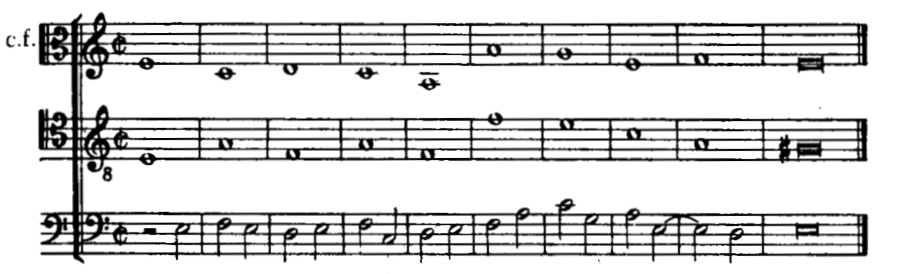
\includegraphics[width=1\textwidth]{Images/Species_examples/2sp-example.png}
    \caption{Example of a second species counterpoint in three-part composition}
    \label{fig:example-2sp}
\end{figure}
\subsection{Formalisation in English}\label{formalisation-en-2nd}
\subsubsection{Harmonic rules}
\begin{enumerate}[wide, label=\bfseries 2.H\arabic*]
\setcounter{enumi}{3} % Start from 4
    \item \textit{Major thirds are now allowed in the last chord.} \label{rule:major-third-last-chord}    
    \begin{quotation}
        "A major third [may] appear in the last chord."
        \textcite[p.87]{GaPEng}
    \end{quotation}
    This is a consequence of now using three voices instead of two. Fux makes explicit two implicit rules we had already defined (\ref{rule:last-chord-not-perfect-anymore} and~\ref{rule:last-chord-h-triad}). It has thus already been implemented in the first species for two voices.

    \item \textit{The half notes must be coherent with respect to the whole notes.} \label{rule:concur-2nd}    
    \begin{quotation}
        "The half notes are always concordant with the two whole notes."
        \textcite[p.88]{GaPEng}
    \end{quotation}
    One might ask what Fux meant when he wrote "concordant". Did he mean to say "consonant"? Our take on the question is that he meant that the half notes are written whilst taking the whole notes into account. This interpretation is aligned with the French translation, and even with the Latin original. In other words, Fux just says "there are constraints on the half notes". It is thus not a rule \textit{per se}.
\end{enumerate}

\subsubsection{Melodic rules}
\begin{enumerate}[wide, label=\bfseries 2.M\arabic*]
\setcounter{enumi}{1} % Start from 4
    \item \greendots \textit{It is allowed to ligate the fourth-to-last with the third-to-last or to ligature the third-to-last with the second-to-last.} \label{rule:2nd-species-ligatures}    
    \begin{quotation}
        "Ligatures have no place in this species [except] in the final cadence."
        \textcite[p.87]{GaPEng}
    \end{quotation}
    Fux explains that in some cases, you have no other option than ligaturing the fourth-to-last and the third-to-last notes. The reasons he gives for this are all part of the previous mentioned rules (no successive perfect consonances, no unison, ...).

    Later on, he also says that the third-to-last and the second-to-last notes can be ligatured (hence producing a whole note).
    \begin{quotation}
        "A whole note may occasionally be used in the next to last measure."
        \textcite[p.93]{GaPEng}
    \end{quotation}
    He says that in the chapter about third species, but it seems that this applies even in cases where the second species is not used in combination with the third (see figures 134, 173 and 174 of the English version).

    He doesn't state clearly if the three of them can get ligatured, but it seems quite obvious that this is not allowed, as it would introduce a lot of redundancy in the composition. It is hence decided that the rule is: a ligature may happen in one case or in the other, but not in both.

    We thus have to relax the already existing constraint from two-part composition stating that no two consecutive notes can be the same, to accept it in some cases.
\end{enumerate}

\subsubsection{Motion rules}
\begin{enumerate}[wide, label=\bfseries 2.P\arabic*]
\setcounter{enumi}{2} 
    \item \texttt{[PREF]} \textit{Successive fifths on the downbeat are only allowed when they are separated by a third on the upbeat.} \label{rule:succ-fifths-flanking-third}    
    \begin{quotation}
        "A half note may, for the sake of the harmonic triad, occasionally make a succession of two parallel fifth acceptable - which can be effected by the skip of a third."
        \textcite[p.86]{GaPEng}
    \end{quotation}
    Fux didn't speak about prohibiting two parallel (i.e. consecutive) fifths in the second species for two voices. That being said, it is indeed prohibited in three parts composition as you cannot have two successive perfect consonances (see rule~\ref{rule:succ-p-cons}). We thus have to relax constraint~\ref{rule:succ-p-cons} in order to accept two successive consonances, when the two successive fifths flank a third. And since the rule on successive perfect consonances is actually a preference, this means that the cost of successive perfect consonances is not applied if those two consonances are fifths and there is a third in between.

\vspace{.5cm}
\begin{minipage}{0.46\textwidth}
    \centering
    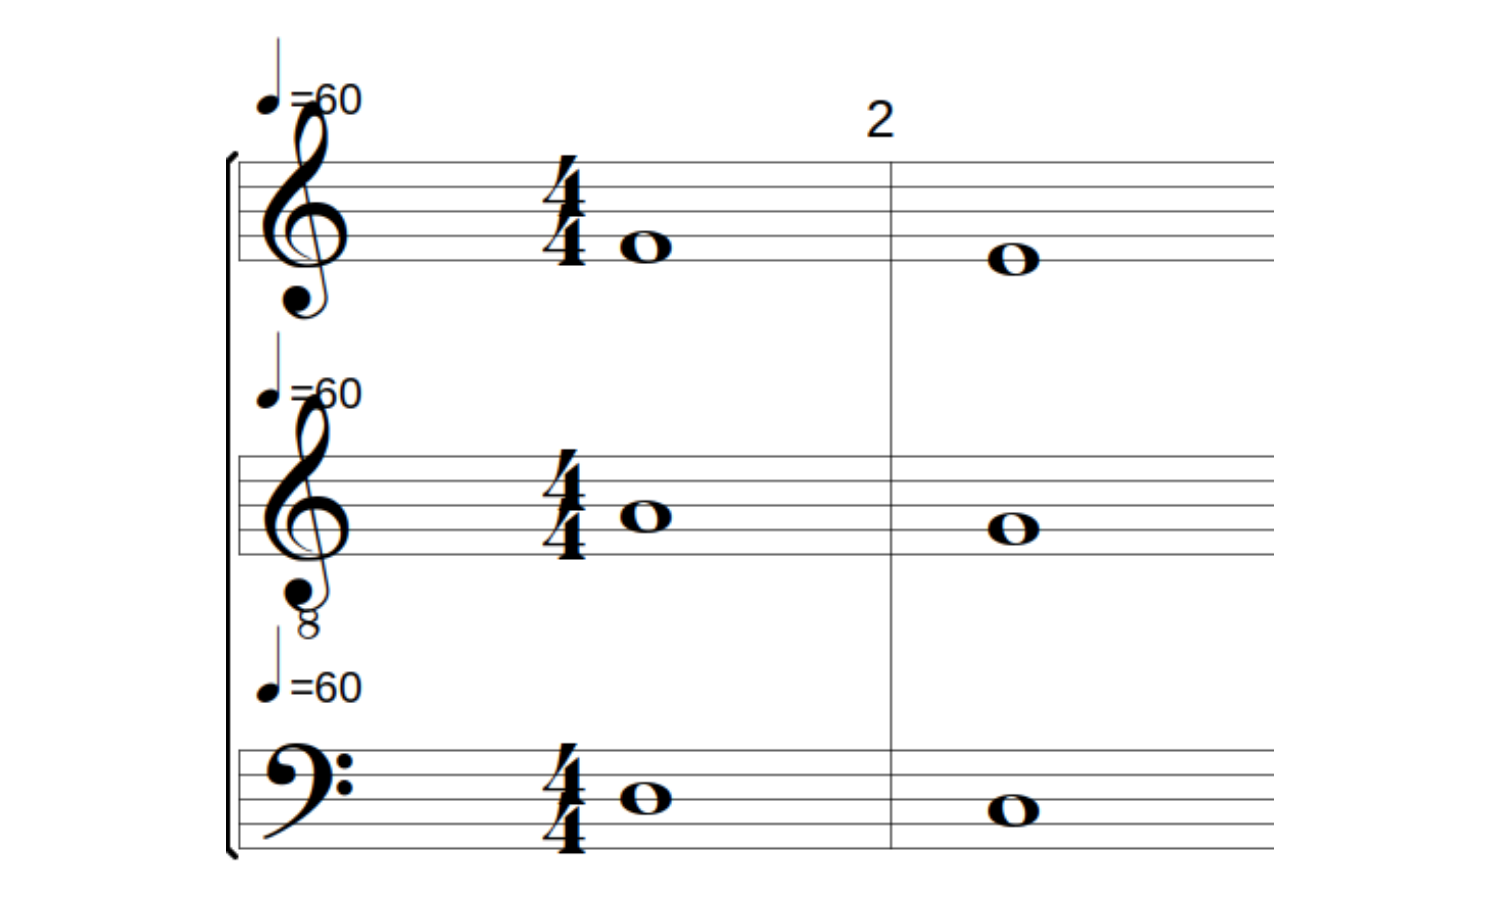
\includegraphics[width=\textwidth]{Images/successive-fifths.png}
    \captionof{figure}{Successive fifths - prohibited}
    \label{fig:successive-fifths-1}
    \end{minipage}
    \hfill
    \begin{minipage}{0.46\textwidth}
      \centering
      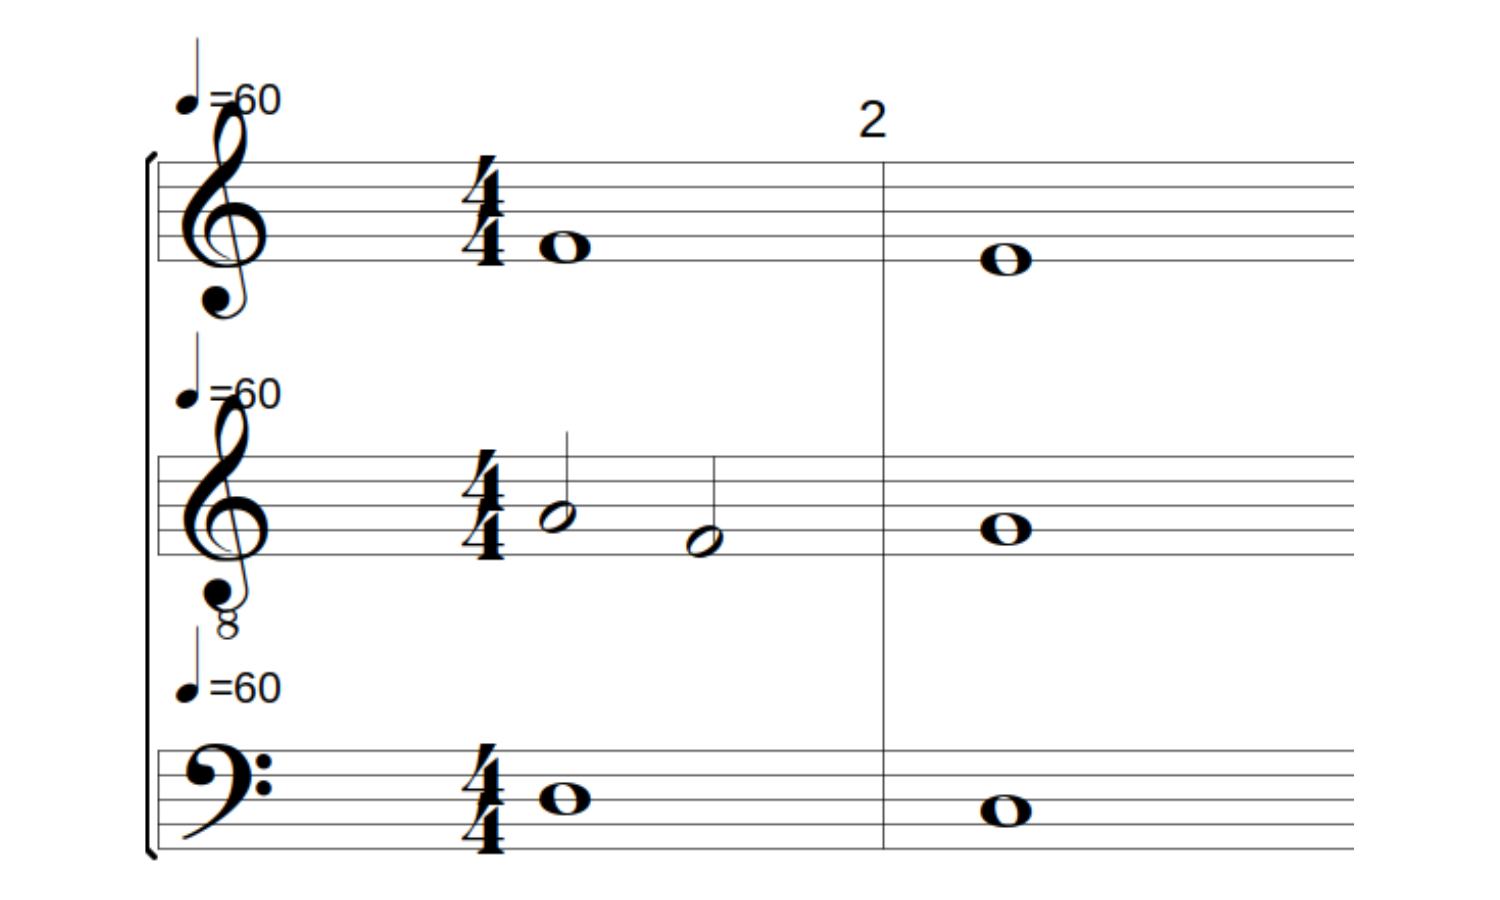
\includegraphics[width=\textwidth]{Images/successive-fifths-flanking-a-third.png}
      \captionof{figure}{Successive fifths separated by a third - valid}
      \label{fig:successive-fifths-2}
\end{minipage}
\end{enumerate}

\subsection{Formalisation into constraints}
\subsubsection{Harmonic rules}
\paragraph{\hspace{.5cm}\ref{rule:major-third-last-chord}} \textit{Major thirds are now allowed in the last chord.}

No need to add a new constraint as this rule is already covered by rules~\ref{rule:last-chord-not-perfect-anymore} and~\ref{rule:harmonic-triad}.

\paragraph{\hspace{.5cm}\ref{rule:concur-2nd}} \textit{The half notes must be coherent with respect to the whole notes.}

No need to add a new constraint as this is not an actual rule.

\subsubsection{Melodic rules}

    \paragraph{\hspace{.6cm}\ref{rule:2nd-species-ligatures}} \greendots \textit{It is allowed to ligate the fourth-to-last with the third-to-last or to ligature the third-to-last with the second-to-last.}  

    This is a relaxation of the two-voice rule \textbf{2.M2} "two consecutive notes cannot be the same".
    
    The reason why this rule has been implemented as a constraint relaxation instead than as a cost is because Fux does not say that ligaturing is bad, he just presents it as a new option offered by the three-part composition.

    \begin{equation}
        \begin{aligned}
            &\forall j \in [1, m), \quad j \neq m-2:\\
            &((N[2, j-1] \neq N[0, j]) \land (N[0, j] \neq N[2, j])) \\
            &\land \\
            & ((N[2, m-3] \neq N[0, m-2]) \lor (N[0, m-2] \neq N[2, m-2]) )
        \end{aligned}
    \end{equation}

    The first line prohibits ligatures except in the positions where they are allowed, and the second line states that only \textit{one} ligature can occur.

\subsubsection{Motion rules}
\paragraph{\hspace{.6cm}\ref{rule:succ-fifths-flanking-third}} \texttt{[PREF]} \textit{Successive fifths on the downbeat are only allowed when they are separated by a third on the upbeat.} 

    This rule is a relaxation of the cost~\ref{rule:succ-p-cons} defined above, and is thus rewritten to correspond to a special case that occurs with the second species.
        
    In the following equation, only $p_1$ must be a second species \cp, $p_2$ can be any species.
    \begin{equation}
        \begin{aligned}
            & \forall p_1, p_2 \in \{\mathit{cf}, cp_1, cp_2\} \text{ where }  p_1 \neq p_2, \quad \forall j \in [0, m-1): \\
            &\mathcal{C}_{succ\_p\_cons} = \,  
            \begin{cases}
                0 & \text{if } (H(p_1, p_2)[0, j] \notin Cons_p) \lor (H(p_1, p_2)[0, j+1] \notin Cons_p)\\
                0 & \text{if } (H(p_1, p_2)[0, j] = 7 ) \land (H(p_1, p_2)[0, j+1] = 7) \\
                & \quad \quad \quad \quad \quad \quad\land (H(p_1, p_2)[2, j] = 3) \lor (H(p_1, p_2)[2, j] = 4)\\
                2 & \text{otherwise } \\
            \end{cases}\\
        \end{aligned}
    \end{equation}

    The meaning of this equation is that $\mathcal{C}_{succ\_p\_cons}$ is equal to zero if one of the two considered consonances is not perfect (because then we do not have two successive perfect consonances), or if we have two successive fifths with a third in between. Otherwise (when we have perfect consonances), the cost must be set.

\section{Third species}
The third species consists only of quarter notes. It introduces even more dissonance than the second species and opens the space for more variation. 

All the rules in this section apply when $species(p) =3$. Note that the rules for the first species also apply to counterpoints of the third species.

\begin{figure}[h]
    \centering
    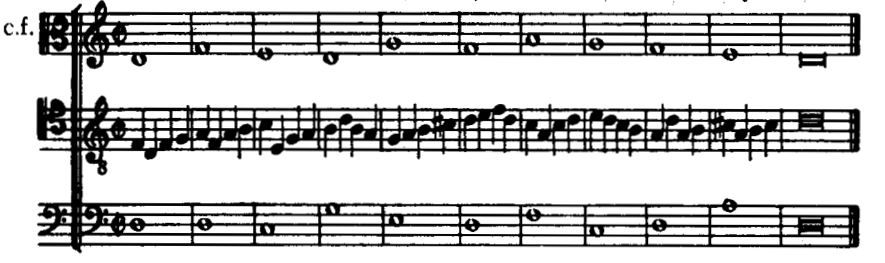
\includegraphics[width=1\textwidth]{Images/Species_examples/3sp-example.png}
    \caption{Example of a third species counterpoint in three-part composition}
    \label{fig:example-3sp}
\end{figure}
\subsection{Formalisation in English}\label{formalisation-en-3rd}
\subsubsection{Harmonic rules}
\begin{enumerate}[wide, label=\bfseries 3.H\arabic*]
\setcounter{enumi}{4}
    \item \textit{The quarter notes must be coherent with respect to the whole notes.} \label{rule:concur-3rd}    
    \begin{quotation}
        "The quarters have to concur with the whole notes of the other voices."
        \textcite[p.91]{GaPEng}
    \end{quotation}
    When Fux uses the word "concur", he most likely means "are related" and not "are consonant". This is the same as for the rule~\ref{rule:concur-2nd} in the second species, where the half notes had to be \textit{concordant} with the \textit{cantus firmus}. This is not a rule in itself, Fux is just saying that some rules should be followed (i.e. the other constraints).

    \item\texttt{[PREF]}  \textit{If the harmonic triad could not be used on the downbeat, it should be used on the second or third beat.} \label{rule:h-triad-3rd-sp}     
    \begin{quotation}
        "Take care whenever you cannot use the harmonic triad on the first quarter occurring on the upbeat, to use it on the second or third quarters."
        \textcite[p.91]{GaPEng}
    \end{quotation}

    This rule is quite clear and speaks for itself.
\end{enumerate}

\subsubsection{Melodic rules}
Fux introduces no new melodic constraints for the third species.
\subsubsection{Motion rules}
Fux introduces no new motion constraints for the third species.

\subsection{Formalisation into constraints}
\subsubsection{Harmonic rules}
\paragraph{\hspace{.5cm}\ref{rule:concur-3rd}} \textit{The quarter notes must be coherent with respect to the whole notes.}

As has been discussed in the previous section, there is no constraint to add for this rule, which isn't really a rule.

\paragraph{\hspace{.6cm}\ref{rule:h-triad-3rd-sp}} \texttt{[PREF]} \textit{If the harmonic triad could not be used on the downbeat, it should be used on the second or third beat.}    

    This rule is quite clear and speaks for itself. Since this is not a strict rule but an advice, it was treated as a cost.

    \begin{equation} \begin{aligned}
            &\forall j \in [0, m) \colon \\
            &(H[1, j] \notin Cons_{h\_triad}) \land  (H[2, j] \notin Cons_{h\_triad})\\
            &\iff \mathcal{C}_{harmonic-triad-3rd-species}[j] = 1       
    \end{aligned} \end{equation}




\section{Fourth species}
As a reminder, the fourth species consists of syncopations. Each note is played on the upbeat and is ligated to the next note on the upbeat.

All the rules in this section apply when $species(p) =4$. Note that the rules for the first species also apply to counterpoints of the third species.

\begin{figure}[h]
    \centering
    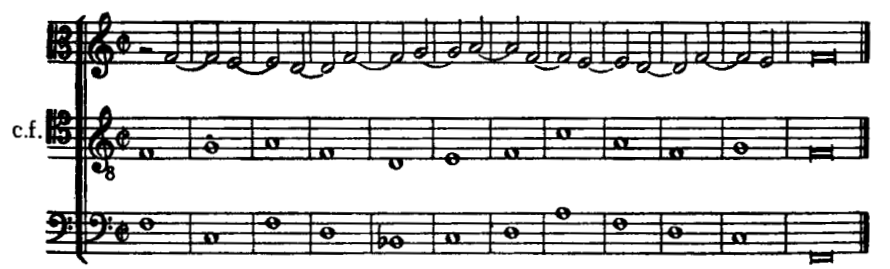
\includegraphics[width=1\textwidth]{Images/Species_examples/4sp-example.png}
    \caption{Example of a fourth species counterpoint in three-part composition}
    \label{fig:example-4sp}
\end{figure}

\subsection{Formalisation in English}\label{formalisation-en-4th}
\subsubsection{Structural constraints}
\begin{enumerate}[wide, label=\bfseries 4.S\arabic*]
\setcounter{enumi}{0}
    \item \textit{The fourth species is staggered by two beats.} \label{rule:delaying}    
    \begin{quotation}
        "The ligature is nothing but a delaying of the note following."
        \textcite[p.95]{GaPEng}
    \end{quotation}
    Fux here insists on a fact that we have already discussed in~\ref{nota-bene-4th-species}. The fourth species behaves as if its upbeats were the downbeats and its downbeats were the upbeats of the previous measure.

    \item \textit{All parts can become the lowest stratum somewhere in the composition.} \label{rule:tenor-might-take-place-of-bass}    
    \begin{quotation}
        "The tenor takes the place of the bass - a thing that not only the tenor may do, but also the alto and even the soprano."
        \textcite[p.100]{GaPEng}
    \end{quotation}
    Fux speaks here about our concept of strata. The tenor can become the lowest stratum, just like the alto and the soprano may do. This is a fundamental concept of the generalization of Fux counterpoint to three voices, and has already been extensively discussed before (see section~\ref{section:parts-and-strata}).
\end{enumerate}

\subsubsection{Harmonic rules}
\begin{enumerate}[wide, label=\bfseries 4.H\arabic*]
    \setcounter{enumi}{4}
    \item \texttt{[PREF]} \textit{Imperfect consonances are preferred over fifth intervals, which in turn are preferred over octaves.} \label{rule:prefer-fifths-over-octaves}    
    \begin{quotation}
        "The fifth is a perfect consonance, the octave a more perfect one, and the unison the most perfect of all; and the more perfect a consonance, the less harmony it has."
        \textcite[p.97]{GaPEng}
    \end{quotation}
    This rule is as clear as it gets.
\end{enumerate}

\subsubsection{Melodic rules}
Fux introduces no new melodic constraints for the fourth species.

\subsubsection{Motion rules}
\begin{enumerate}[wide, label=\bfseries 4.P\arabic*]
\setcounter{enumi}{2}
    \item \texttt{[PREF]} \textit{Successive fifths are allowed when using ligatures.} \label{rule:successive-fifths-in-4th-species}    
    \begin{quotation}
        "[It would be impossible to remove] the ligatures because of another consideration, the immediate succession of several fifths."
        \textcite[p.95]{GaPEng}
    \end{quotation}
    By saying that it exists a rule that prohibits the succession of fifths (which is actually just a particular case of rule~\ref{rule:succ-p-cons}, stating that you cannot have two successive perfect consonances) when there is no ligature, Fux is telling us in an indirect way that this rule is not applicable when there are ligatures. He further complements by saying "there is great power in ligatures - the ability to avoid or improve incorrect passages".
    
    The conclusion is that successive fifths are allowed in the fourth species.

    \item \texttt{[PREF]} \textit{Resolving to a fifth is preferred over resolving to an octave.} \label{rule:resolving-to-fifths-rather-than-octaves}    
    \begin{quotation}
        "A dissonance that resolves to a fifth is more acceptable than a dissonance that resolves to an octave."
        \textcite[p.98]{GaPEng}
    \end{quotation}
    This rule could not be clearer.
    
    \item \textit{Stationary movement in the bass implies dissonance in the fourth species part.} \label{rule:dissonance-in-4th-species}
    \begin{quotation}
        "If I said that the first note of the ligature must always be consonant, that applies only to the instances in which the lower voice moves from bar to bar, but not the instances in which the bass remains on a pedal point, that is, in the same position. In such a case a ligature involving only dissonances is not only correct but even very beautiful."
        \textcite[p.98]{GaPEng}
    \end{quotation}
    The rule evoked here cancels the previous rule \textbf{4.H1W} that stated that all notes should be consonant. From now on, if the lowest stratum has a stationary movement, the corresponding delayed note in the fourth species must be a dissonance, instead of a consonance.    


    \item \textit{A note provoking a hidden fifth gets replaced by a rest.} \label{rule:hidden-fifths}
    \begin{quotation}
        "Here a hidden succession of fifths occurs, which is easily perceptible to the ear and should be avoided in three part composition. This may be managed by using a rest."
        \textcite[p.98]{GaPEng}
    \end{quotation}
    Fux's uses the term 'hidden succession of fifths' without any prior definition. It is therefore difficult to be sure of what he meant, since the traditional terms for such progressions are as vague and variable as the traditional rules that govern them. Nevertheless, many authors seem to agree on the following definition of a 'hidden interval': a hidden fifth or hidden octave is when you approach a perfect fifth or perfect octave by direct motion. \cite[p.31]{piston1987harmony}. Looking closely at figures 137, 151 and 152 of the English version of \gap, this definition is consistent with Fux's interpretation.

    The point of the rule then is: if a solution leads to a hidden fifth, then the note that provokes the fifth is replaced by a rest. This rule is an \textit{a posteriori} rule: it applies after the solution has been found.
    The current rule thus complements the rule~\ref{rule:successive-fifths-in-4th-species} (about successive fifths in fourth species) and the rule~\ref{rule:direct-to-p-cons} (about direct moves to perfect consonances) without changing them.
    
    See figures~\ref{fig:hidden-fifths-1} and~\ref{fig:hidden-fifths-2}:

    \begin{figure}[h]
        \centering
        \begin{minipage}{0.49\textwidth}
            \centering
            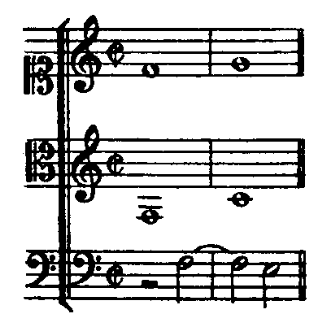
\includegraphics[width=.4\textwidth]{Images/hidden-fifths-1.png}
            \caption{Invalid solution featuring hidden fifths}
            \label{fig:hidden-fifths-1}
        \end{minipage}
        \hfill
        \begin{minipage}{0.49\textwidth}
            \centering
            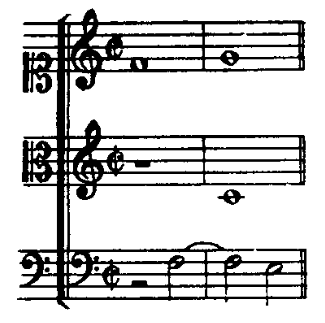
\includegraphics[width=.4\textwidth]{Images/hidden-fifths-2.png}
            \caption{Valid solution replacing the hidden fifth by a rest.}
            \label{fig:hidden-fifths-2}
        \end{minipage}
    \end{figure}

\end{enumerate}

\subsection{Formalisation into constraints}\label{formalisation-c-4th}
\subsubsection{Structural constraints}
    \paragraph{\hspace{.5cm}\ref{rule:delaying}} \textit{The fourth species is staggered by two beats.}

    There is no constraint to add since this rule is the very definition of the fourth species.

    \paragraph{\hspace{.5cm}\ref{rule:tenor-might-take-place-of-bass}} \textit{All parts can become the lowest stratum somewhere in the composition.} 
    
    Again, there is no constraint to add since this rule is already covered by the concept of lowest stratum.


\subsubsection{Harmonic rules}
\paragraph{\hspace{.6cm}\ref{rule:prefer-fifths-over-octaves}} \texttt{[PREF]} \textit{Imperfect consonances are preferred over fifth intervals, which in turn are preferred over octaves.}   

    This rule is almost covered by the existing costs (see~\ref{rule:prefer-imp-to-perf-appendix}), as a perfect consonance has a higher cost than an imperfect consonance. But Fux says not only that imperfect consonance should be preferred over perfect ones, he says that fifths should be preferred over octaves. This precision in the rule (fifth is better than octave) could be solved by either putting a higher cost to octaves and lower one to fifths, or to put the cost for fifth before the cost for octaves in the lexicographical array of costs, but this is discussed in the parts about costs (see~\ref{costs}).


\subsubsection{Motion rules}
In this subsection, the correct notation is used for the species (see \ref{nota-bene-4th-species}). So X[0,0] actually means X[0,0], and not X[2,0] as in other parts.

\paragraph{\hspace{.6cm}\ref{rule:successive-fifths-in-4th-species}} \texttt{[PREF]} \textit{Successive fifths are allowed when using ligatures.}    

    The point of this rule is that Fux introduces an exception to~\ref{rule:succ-p-cons}: successive fifths are allowed in the fourth species.

    We shall then amend the rule~\ref{rule:succ-p-cons} (don't forget that it is a cost) to allow successive fifths in any case, and rewrite it as:
    \begin{equation} \begin{aligned}
        &\forall p_1, p_2 \in \{\mathit{cf}, cp_1, cp_2\}, \quad \text{with } p_1 \neq p_2, \quad \forall j \in [0, m-1) \colon\\
        &\mathcal{C}_{succ\_p\_cons} = \,  
        \begin{cases}
            0 & \text{if } (H(p_1, p_2)[2, j] \notin Cons_p) \lor (H(p_1, p_2)[2, j+1] \notin Cons_p)\\
            0 & \text{if } (H(p_1, p_2)[2, j] = 7) \land (H(p_1, p_2)[2, j+1] = 7) \\
            2 & \text{otherwise } \\
        \end{cases}\\
    \end{aligned} \end{equation}

    The meaning of this equation is that the cost is set to zero if the two consecutive intervals are not perfect consonances, or if the consecutive intervals are both fifths. Otherwise, the cost must be set.

    \paragraph{\hspace{.6cm}\ref{rule:resolving-to-fifths-rather-than-octaves}} \texttt{[PREF]} \textit{Resolving to a fifth is preferred over resolving to an octave.}    
    
    This is already covered by the rule~\ref{rule:prefer-fifths-over-octaves} (prefer fifths over octaves), since preferring fifths over octaves in \textit{all} cases implies preferring to resolve to a fifth rather than to an octave.

    \paragraph{\hspace{.6cm}\ref{rule:dissonance-in-4th-species}} \textit{Stationary movement in the bass implies dissonance in the fourth species part.}

    \begin{equation}
        \begin{aligned}
        &\forall j \in [0, m-1):\\
        &M(a)[0, j] \neq 0 \iff H[2, j] \in Cons\\
        &M(a)[0, j] = 0 \iff H[2, j] \in Dis
        \end{aligned}
    \end{equation}        


    \paragraph{\hspace{.6cm}\ref{rule:hidden-fifths}} \textit{A note provoking a hidden fifth gets replaced by a rest.}
    \begin{equation}
        \begin{aligned}
            &\forall j \in [1, m-1):\\
            &H[0, j] = 7 \land P[0,j] = 2 \iff N[0, j-1] = \emptyset  
        \end{aligned}
    \end{equation}

    This rule is very special because it applies after the search, not during the search. More precisely, after the search is started and a result is found, only then does this rule begin to apply. To understand why, remember that the suppressed note is suppressed because it causes a hidden fifth. But the only way to have a hidden fifth is to have an existing note, you cannot have a hidden fifth to a non-existing note. So we don't delete the note during the search, because then we would also delete the hidden fifth (because you can't have a hidden fifth without a note) and so we would change the solution. You have to find a solution first, and then remove the possible note that causes a hidden fifth. 

    This is actually a very interesting property, because here we have a note that is not played and yet has an effect on the composition.



\section{Fifth species}

As a reminder, the fifth species is a mix of all previously mentioned species, which means that it combines the rules from all previous species.

\begin{figure}[h]
    \centering
    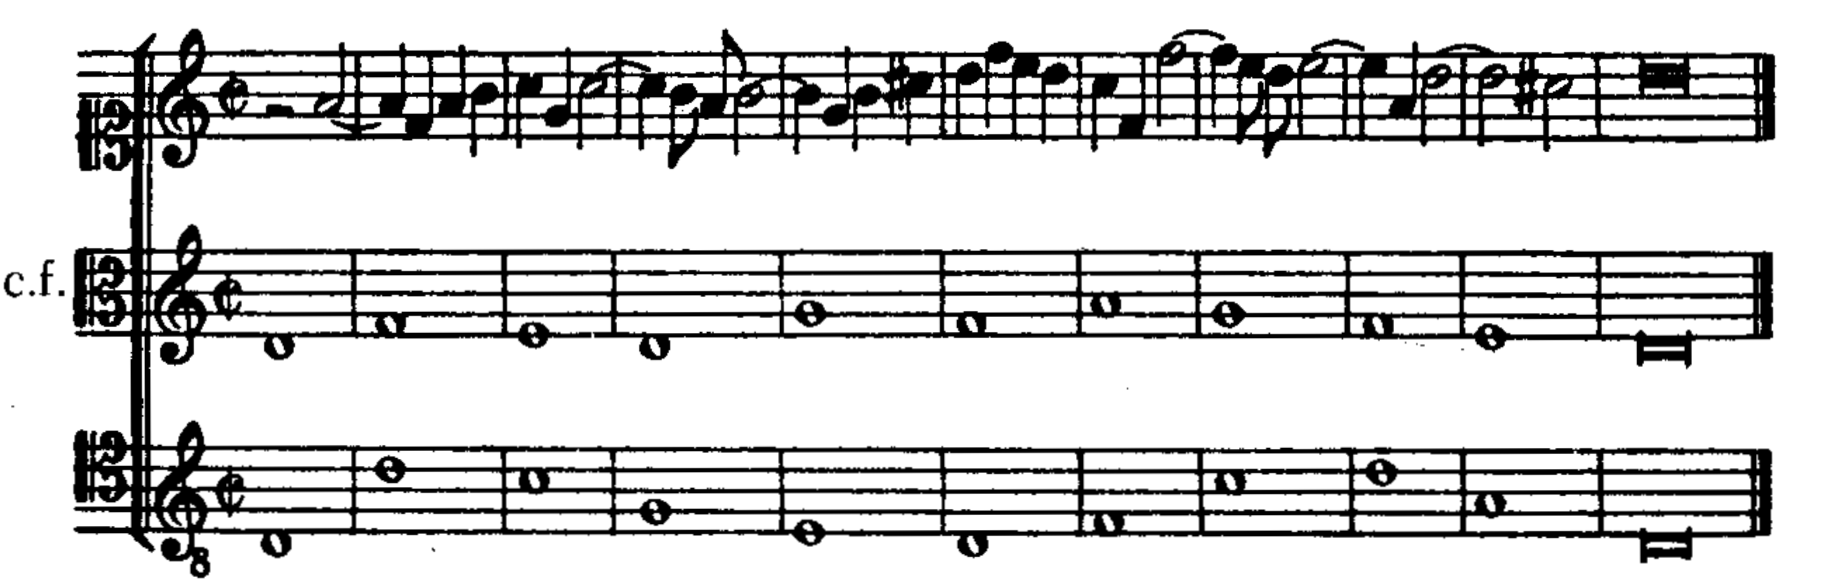
\includegraphics[width=1\textwidth]{Images/Species_examples/5sp-example.png}
    \caption{Example of a fifth species counterpoint in three-part composition}
    \label{fig:example-5sp}
\end{figure}

\paragraph{}
No additional rules (be they harmonic rules, melodic rules or motion rules) were observed by Fux when writing a three-part counterpoint with the fifth species.


However, in order to have some rhythmic variety when composing with two fifth species counterpoints, it was decided to impose a rule that Fux never mentioned. We know that the fifth is just all the other species combined, and the way the solver understands this is that it considers each note of the composition to belong to a particular species. This is represented as S[i,j], where $S[i,j]=x$ means that the i-th note of the j-th measure belongs to the x-th species. So if $S(cp_1)[2, 3]=3$, then the second note of the third measure of the first counterpoint is constrained by the constraints of the third species. From the solver's point of view, $S$ is just an array like all the others, but it branches on it during the search to guarantee that the composition of the fifth species is composed of as many species as possible.

This gives us a metric for similarity, since two fifth-species counterpoints that have the same $S$ array will be rhythmically redundant. To tackle this problem, we force the solver to find a solution where $S(cp_1)$ must be at least half as different as $S(cp_2)$. 

\noindent
\begin{minipage}{0.37\textwidth}
    As can be seen in Figure \ref{fig:fifth-species-redundancy}, the first composition is indeed rhythmically redundant, since both fifth-species counterpoints have (almost) the same rhythm. The second is much less redundant, since it was required that the counterpoints use different species for at least 50\% of the beats.
    \end{minipage}
    \hfill
    \begin{minipage}{0.6\textwidth}
      \centering
      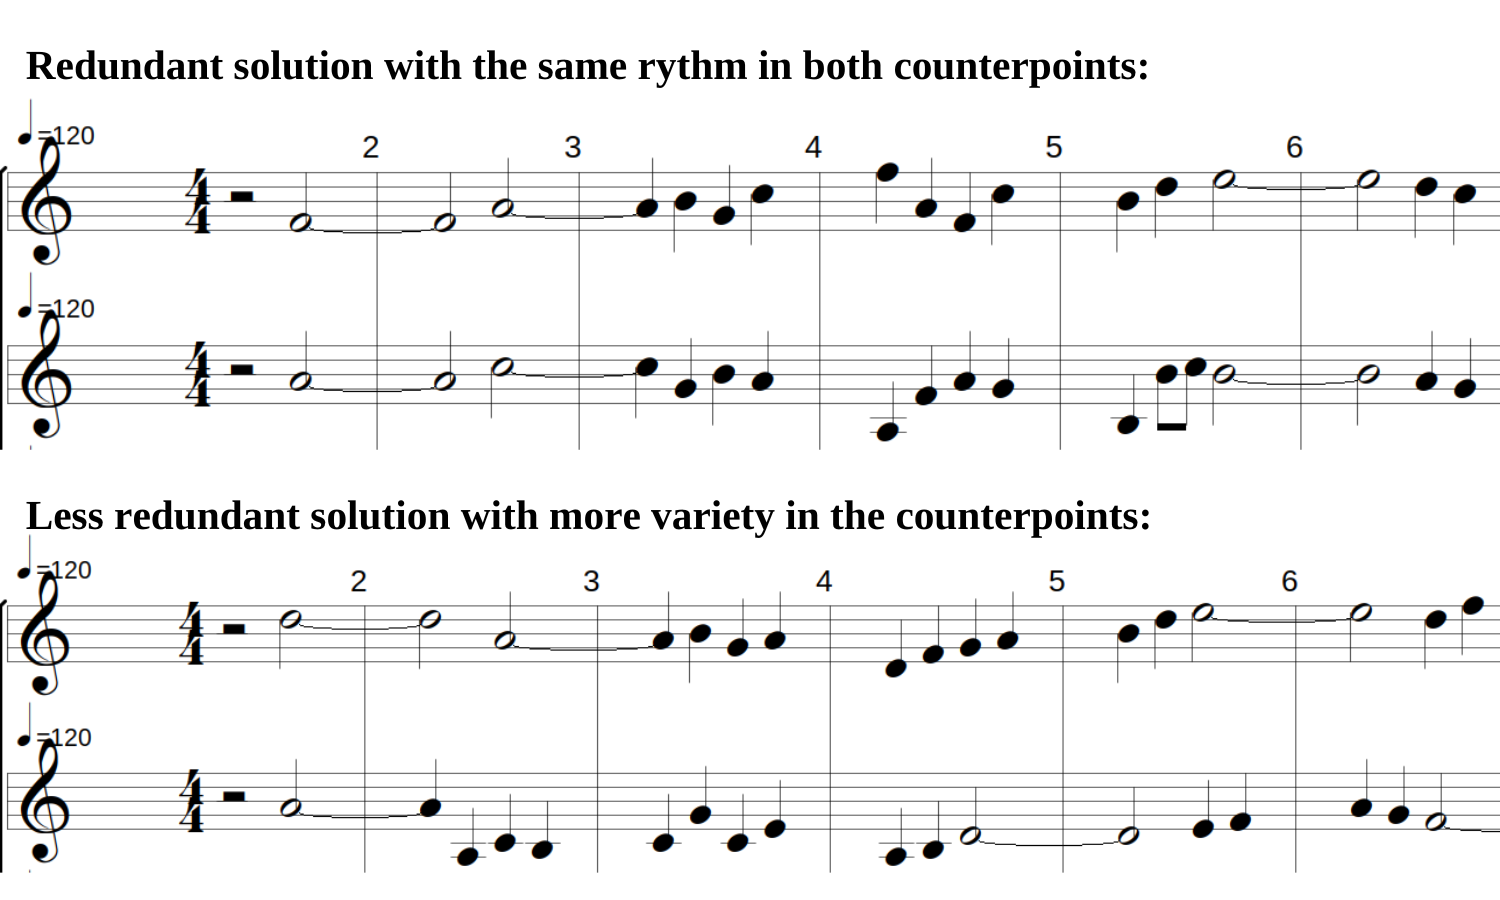
\includegraphics[width=\textwidth]{Images/fifth-species-redundancy.png}
      \captionof{figure}{Two compositions of two fifth-species counterpoint, one redundant and the other not}
      \label{fig:fifth-species-redundancy}
\end{minipage}
\vspace{.5cm}


\begin{equation}
\begin{aligned}
 \mathit{species(cp_1)} = \mathit{species}(cp_2) = 5 \iff \sum_{i=0}^{3} \sum_{j=0}^{m-1} (S(cp_1)[i,j] = S(cp_2)[i,j]) < \frac{s_m}{2}
\end{aligned}
\end{equation}

This equation is only true if both counterpoints are of the fifth species, and its meaning is that the sum of the times $S(cp_1)=S(cp_2)$ must be less than half the number of notes in the composition.

\section{Writing a three-part composition using various species}
In \gap, Fux almost always writes his counterpoints using a combination of the first species and another species, i.e. he makes the following combinations: 1+1, 1+2, 1+3, 1+4, 1+5. Only sometimes does he make other combinations, either with two counterpoints of the same type (5+5) or with two different types (2+3).

When creating combinations of different species, Fux doesn't give any specific rules for combining them. It seems that the different species interact with each other as they would do with the first species, taking into account only the first beat of the measure. For example, if we compute a first counterpoint belonging to the 3rd species and a second counterpoint belonging to the second species, the rules that apply between the two counterpoints will be set between all the beats of the first counterpoint and the first beat of the second counterpoint and between all the beats of the second counterpoint and the first beat of the first counterpoint. This corresponds to what we would have done if we had applied the rules between a counterpoint and the \cf, where the rules apply between all beats of the \cfs and the first beat of the counterpoint.

Below is a brief summary of the rules that apply to each species:
\begin{itemize}
    \item \textbf{First species} --- rules of the first species,
    \item \textbf{Second species} --- rules of the first species + rules of the second species,
    \item \textbf{Third species} --- rules of the first species + rules of the third species,
    \item \textbf{Fourth species} --- rules of the first species + rules of the fourth species,
    \item \textbf{Fifth species} --- rules of all species, selected according to the S array.
\end{itemize}
This means that in a composition with two counterpoints, one of the 2nd species and one of the 3rd species, the first counterpoint will follow the rules of the 1st and the 2nd species, and the second counterpoint will follow the rules of the 1st and the 3rd species.